\begin{center}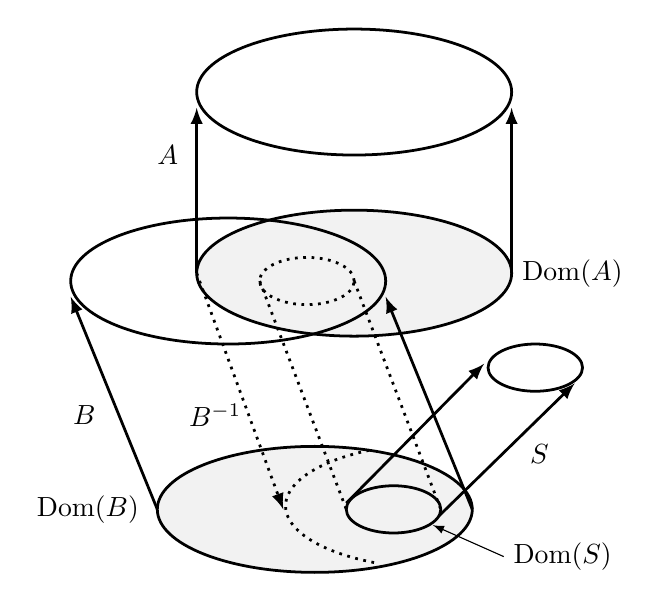
\begin{tikzpicture}
[line width=1pt]
\node at  (1.6+2, 0.1) [right] {$\textrm{Dom}(A)$};
\draw[fill=black!5] (1.6, 0.1) ellipse (2cm and 0.8cm); %% Dom A
\draw               (1.6, 2.4) ellipse (2cm and 0.8cm); %% Img A
\draw[-latex] (1.6+2, 0.1)--(1.6+2, 2.4-.2); %% A right
\draw[-latex] (1.6-2, 0.1)--(1.6-2, 2.4-.2); %% A left
\node at  (1.6-2-.1, 1.6) [left] {$A$};
%%
\node at (1.1-2-.1, -2.9) [left] {$\textrm{Dom}(B)$};
\draw[fill=black!5] (1.1, -2.9) ellipse (2cm and 0.8cm); %% Dom B
\draw               (0  ,  0)   ellipse (2cm and 0.8cm); %% Img B
\draw[-latex] (1.1+2, -2.9)--(0+2, 0-.2); %% B right
\draw[-latex] (1.1-2, -2.9)--(0-2, 0-.2); %% B left
\node at  (0.55-2-.1, -1.7) [left] {$B$};
\draw[-latex,dotted] (1.6-2, 0.1)--(0.7, -2.9); %% B-1
\node at (0.3, -1.7) [left] {$B^{-1}$};
\draw[dotted] (1.79, -2.15) arc(118:244: 2cm and 0.8cm); %% Arc
\draw[dotted] (1, 0) ellipse (0.6cm and 0.3cm); %% Dotted S
\draw         (2.1, -2.9) ellipse (0.6cm and 0.3cm); %% Dom S
\draw[dotted] (1-0.6, 0)--(2.1-0.6, -2.9); %% B-1
\draw[dotted] (1+0.6, 0)--(2.1+0.6, -2.9); %% B-1
\draw                     (3.9, -1.1) ellipse (0.6cm and 0.3cm); %% Img S
\draw[-latex] (2.1-0.6, -2.9+.08)    --(3.9-0.6-.05, -1.1+.05); %% Left S
\draw[-latex] (2.1+0.6-.02, -2.9-.08)--(3.9+0.6-.1, -1.1-.2); %% Right S
\node at  (3.7,-2.2) [right] {$S$};
\draw[-latex,thin] (3.5, -3.5) node[right]{$\mathrm{Dom}(S)$} -- (2.1+0.5, -2.9-0.2);
\end{tikzpicture}\end{center}
